\documentclass{article}

% Official NeurIPS 2025 style (the 2027 style is not released yet; swap the file and the
% option when it is). Anonymous submission by default; use [final] or [preprint] otherwise.
\usepackage[preprint]{neurips_2025}

\usepackage[utf8]{inputenc}
\usepackage[T1]{fontenc}
\usepackage{lmodern}
\usepackage{hyperref}
\usepackage{url}
\usepackage{booktabs}
\usepackage{amsmath,amssymb,amsthm,amsfonts}
\usepackage{nicefrac}
\usepackage{microtype}
\usepackage{xcolor}
\usepackage{graphicx}
\usepackage{algorithm}
\usepackage{algpseudocode}
\usepackage[capitalise,noabbrev]{cleveref}

\newtheorem{theorem}{Theorem}
\newtheorem{lemma}{Lemma}
\newtheorem{corollary}{Corollary}
\newtheorem{proposition}{Proposition}
\theoremstyle{definition}
\newtheorem{definition}{Definition}

\title{Knowing When You're Done: Termination Detection for\\Recurrent Latent Reasoners under Depth Shift}

\author{%
  Md Fahim Sarker\\
  \texttt{(affiliation and e-mail)}
}

\begin{document}

\maketitle

\begin{abstract}
Recurrent latent reasoners can solve harder problems by iterating for longer, but the extra compute
only helps if the model also knows when to stop. We study this termination problem in a setting where
the answer to ``is the computation finished?'' is known exactly. For local recurrent models, a
light-cone argument assigns every input $x$ a lower bound $\LB(x)$ on the first step at which its answer
can be certified; the bound grows with depth rather than length, and a local, size-invariant automaton
attains it at every length. We introduce DepthShift, a benchmark with exact per-instance depth and
splits that vary depth and length independently, and evaluate fifteen stopping rules on one backbone
family. Jointly trained pooled gates (ACT, PonderNet, TRM-style heads) leak length: on deeper addition
inputs ACT is 99.8\% accurate while halting before $\LB(x)$ through a global shortcut, yet only 35.9\%
once inputs are also longer. Convergence rules stop before the bound on most deep inputs and are still
correct, so premature stopping and premature error must be measured separately. On addition,
per-position confidence halts at exactly $\LB(x)$ on every split, and the local completion heads we
propose match it without improving on it; on segmented parity the same heads learn the training clock
instead. Termination detection beyond the training depth appears to be limited less by the readout than
by training data that never show an unfinished computation at a late step. Code, frozen splits and all
runs are released.
\end{abstract}

\section{Introduction}
\label{sec:intro}

A recurrent or looped model applies the same block again and again, and every extra iteration buys more
computation on the same input. This lets small networks extrapolate to instances harder than any seen
in training, provided they are allowed to think for longer
\citep{schwarzschild2021thinking,bansal2022endtoend,geiping2025scaling,jolicoeur2025trm}. The promise is
adaptive compute, with few steps on easy inputs and many on hard ones, and keeping it requires a
stopping rule. The rules in common use, learned halting gates \citep{graves2016act,banino2021pondernet},
confidence thresholds and convergence tests \citep{zhou2020pabee,geiping2025scaling}, are all fitted on
the difficulty seen in training. Yet the inputs that matter most are the ones harder than anything in
the training set, and on them the rule must decide that the computation is finished from information it
was never rewarded for reading.

We study this decision in a setting where the right answer is known. In a \emph{local} recurrent
reasoner, one step moves information by at most $r$ positions, so after $t$ steps position $i$ depends
only on the input within radius $rt$, its light cone. If that window does not yet determine the target,
some other input agrees on the window but has a different answer, and the model must be wrong on one of
the two. Every input therefore has a lower bound $\LB(x)=\ceil{\dstar(x)/r}$ on the first step at which
its answer can be certified (\cref{thm:lb}), where the \emph{depth} $\dstar(x)$ is the largest radius any
position needs. Halting earlier returns an answer that the model's own state does not determine, correct
only by luck of the data. Because the bound depends on depth and not on length, it separates two shifts
that are usually confounded, longer inputs and deeper ones. For the tasks we study, a constant-size local
automaton halts at exactly $\LB(x)$ at every length (\cref{prop:automaton}), so the bound is attainable
and we can ask which stopping rules attain it.

Our contributions are threefold. We prove the light-cone bound, which turns ``halting too early'' into a
checkable per-instance quantity, derive its consequences for local commit-on-done rules and for rules
that see only the length, and give closed-form depth oracles and a matching automaton for addition and
segmented parity, each with an executable test (\cref{sec:theory}). We introduce DepthShift, whose
frozen splits vary depth and length independently up to $12.8\times$ the training depth
(\cref{sec:benchmark}). And we evaluate fifteen stopping rules and four references on one backbone family,
from post-hoc confidence and convergence tests through ACT, PonderNet and pooled TRM-style and v1 heads to
a family of local \emph{completion heads} that we introduce, scoring each by accuracy, steps, and how often
it stops or errs before $\LB(x)$ (\cref{sec:method,sec:experiments}).

The results tell a consistent story. Jointly trained pooled gates leak length: on addition, ACT is
99.8\% accurate on deeper inputs with fewer steps than the bound allows, because it reads a global
shortcut, and falls to 35.9\% once inputs are both deeper and longer. Premature stopping and premature
error are different things: convergence rules halt before the bound on most deep addition inputs and
are still right, because a travelling carry keeps the hidden state moving until it lands. When pending
positions are genuinely ambiguous, as in addition, per-position confidence is already a certificate;
max-softmax halts at exactly $\LB(x)$ on every split, and our completion heads match it without improving
on it. When they are not, as in parity, the completion heads learn the training clock, while pooled gates
extrapolate in depth but fall below 1\% once inputs are also longer. Finally, jointly trained completion
heads leave the backbone's solution intact, whereas gates that reweight the task loss degrade it. The
difficulty of termination detection thus lies less in the readout than in training data that never show
a computation still unfinished at a late step.

\section{Setup and theory}
\label{sec:theory}

\paragraph{Local recurrent reasoners.}
An input is a sequence $x = (x_0,\dots,x_{P-1})$ over an alphabet $\Sigma$, and the task assigns an
output $y_i(x)\in\Gamma$ to every position. Positions outside $\{0,\dots,P-1\}$ hold a fixed padding
symbol $\bot$; we write $\tilde x$ for the padded sequence. A \emph{local recurrent reasoner} with
growth rate $r$ keeps one latent vector per position and computes
\begin{equation}
  e_i = E(x_i),\quad h_i^{(0)} = H(e_i),\quad
  h_i^{(t+1)} = U\big(h^{(t)}_{i-r:i+r},\, e_{i-r:i+r}\big),\quad
  \hat y_i^{(t)} = D\big(h_i^{(t)}\big),
  \label{eq:local}
\end{equation}
where $E, H, D$ are pointwise, $U$ is shared across positions and steps, and $h_j, e_j$ outside the
input take fixed padding values. Our backbone (\cref{sec:method}) is an instance with
$r$ kernel-3 convolutions per step. Write $W_i^{\rho}(x) = (\tilde x_{i-\rho},\dots,\tilde x_{i+\rho})$
for the window of radius $\rho$ around $i$, including padding symbols.

\begin{lemma}[Light cone]\label{lem:cone}
For every $t\ge 0$, $h_i^{(t)}$ is a function of $W_i^{rt}(x)$ only, and this function does not
depend on $i$. Hence if $W_i^{rt}(x) = W_{i'}^{rt}(x')$ then $\hat y_i^{(s)}(x) = \hat y_{i'}^{(s)}(x')$
for all $s\le t$.
\end{lemma}

\paragraph{Per-instance depth.}
The window is all a position can have seen, so the right notion of difficulty is how large a window
must be before the answer is pinned down.

\begin{definition}[Determining radius and depth]\label{def:depth}
Position $i$ of $x$ is \emph{$\rho$-determined} if every pair $(x', i')$ with
$W_{i'}^{\rho}(x') = W_i^{\rho}(x)$ has $y_{i'}(x') = y_i(x)$. The determining radius
$\rho_i(x)$ is the smallest such $\rho$, and the depth of the instance is
$d^*(x) = \max_i \rho_i(x)$.
\end{definition}

Because windows are compared at any position $i'$, the definition matches what a
translation-equivariant model can know: it can see the input boundary only once $\bot$ enters its
window.

\begin{theorem}[Light-cone lower bound and unsoundness]\label{thm:lb}
Let $f$ be any local recurrent reasoner with growth rate $r$, and let $t < \lceil \rho_i(x)/r\rceil$.
Then there is a pair $(x', i')$ with $\hat y_{i'}^{(t)}(x') = \hat y_i^{(t)}(x)$ but
$y_{i'}(x') \ne y_i(x)$. So at step $t$ the model is wrong at position $i$ of $x$ or at position $i'$
of $x'$. In particular, no local reasoner can be correct on every input at a step earlier than
$\mathrm{LB}(x) = \lceil d^*(x)/r\rceil$.
\end{theorem}

The theorem constrains what any \emph{stopping rule} can achieve: halting $x$ at step
$\tau(x) < \mathrm{LB}(x)$ returns an answer that is not certified by the information the model holds.
Whether that answer is wrong depends on which member of the pair the data contain. Two consequences
make this concrete.

\begin{corollary}[Commit-on-done local rules]\label{cor:local}
Suppose each position $i$ raises a done flag that depends only on its own history
$h_i^{(0)},\dots,h_i^{(t)}$, and commits $\hat y_i^{(t)}$ when it does. If the system is correct on
every input, then position $i$ of $x$ commits no earlier than $\lceil \rho_i(x)/r\rceil$, and the input
halts no earlier than $\mathrm{LB}(x)$.
\end{corollary}

\begin{corollary}[Rules that see only the length]\label{cor:length}
For addition, $d^*$ ranges over $\{1,\dots,L+1\}$ at length $L$. A rule whose halting step depends
only on $L$ is correct on every input of length $L$ only if $\tau(L)\ge \lceil (L+1)/r\rceil$.
It then spends $\lceil (L+1)/r\rceil - \mathrm{LB}(x)$ extra steps on every input; for uniformly random
digits $d^* = O(\log L)$ with high probability, so the waste is $\Theta(L)$ steps.
A length-only rule fitted on training depths ($\tau(L) < \lceil (L+1)/r\rceil$) is instead wrong on
one member of every flip pair with $d^* > r\,\tau(L)$.
\end{corollary}

\paragraph{The bound is achievable with local, size-invariant signals.}
For our two exact tasks, the determining radius has a closed form, and a local automaton reaches
the bound for every input length.

\begin{proposition}[Depth oracles]\label{prop:oracles}
\emph{Addition} (digits least-significant first, outputs at positions $0,\dots,L$ with position $L$ the
carry): let a \emph{stop} be a position $j<L$ with $a_j+b_j\ne 9$. Then
$\rho_i(x) = i - s_i$, where $s_i$ is the nearest stop before $i$, or $-1$ if there is none.
Thus $d^*(x)$ is the largest gap between consecutive elements of $\{-1\}\cup\{\text{stops}\}\cup\{L\}$.
\emph{Segmented parity}: $\rho_i(x) = i - s_i$ for non-delimiter $i$, where $s_i$ is the previous
delimiter or $-1$; $d^*(x)$ is the longest run of non-delimiters.
\end{proposition}

\begin{proposition}[Achievability]\label{prop:automaton}
For addition and segmented parity there is a local reasoner with $r=1$ and a commit-on-done local
flag such that, for every input of every length, every committed answer is correct and the input
halts at exactly $\mathrm{LB}(x) = d^*(x)$ steps.
\end{proposition}

The automaton behind \cref{prop:automaton} stores one bit of \emph{pending} state per position (is my
carry-in, or my segment prefix, known yet?) and flips it when a resolved neighbour passes its value
along. Its done flag is a pointwise function of its state, and the same rule works at every length.
This is the inductive bias our completion heads target. A pooled gate or a global confidence
statistic, in contrast, has no reason to wait for the slowest pending chain. \Cref{sec:experiments}
tests whether learned signals behave like the automaton beyond the training depth.

\paragraph{Mazes.} For mazes the determining radius has no closed form, and information must travel
along corridors rather than straight lines, so the light cone gives only a loose bound. We use the
optimal path length and the dead-end-filling depth as empirical depth proxies.

All proofs are in \cref{app:proofs}. Each result has an executable check in
\texttt{tests/test\_theory.py}: the flip test for \cref{lem:cone} on random backbones, the pair
construction of \cref{thm:lb}, brute-force verification of \cref{prop:oracles}, and the automata
of \cref{prop:automaton} on lengths up to 512.

\section{The DepthShift benchmark}
\label{sec:benchmark}

DepthShift pairs tasks that have an exact per-instance depth oracle with a split design that
separates \emph{longer} inputs from \emph{deeper} ones (\cref{fig:splits} in \cref{app:results}). All generators run on the GPU
from fixed seeds. Test sets are frozen and stored with SHA-256 hashes, and the training sampler
discards any instance whose hash matches an in-distribution validation or test instance.

\paragraph{T1: addition.} Each instance consists of two $L$-digit numbers $a$ and $b$, written
least-significant digit first and encoded as one token $10a_i+b_i$ per position, plus one extra position
for the final carry. By \cref{prop:oracles}, the depth is one plus the longest run of digit pairs that
sum to~9, because a carry generated at a stop must ripple through the whole run before the positions
behind it are determined. Uniformly random digits make long runs exponentially rare (each pair sums
to~9 with probability $1/10$), so we control $\dstar$ directly. The generator inserts exactly one run of
length $\dstar-1$ between two stops, draws background runs at a random density, and caps them below
$\dstar-1$. Stops are drawn uniformly from the 90 pairs with $a+b\ne 9$, which means a run receives an
incoming carry with probability $1/2$.

\paragraph{T2: segmented parity.} The input is a bit string interleaved with delimiter tokens, and the
target at each position is the parity of the current segment up to that position. The depth is the
length of the longest segment. Parity differs from addition in a way that turns out to matter: as
information arrives from the left, the intermediate predictions keep flipping, so the per-step outputs
do not settle early.

\paragraph{T3: mazes.} We also generate $n\times n$ mazes with a randomized depth-first search; the
input channels mark open cells, the start and the goal, and the target is the shortest path. We
record the optimal path length and the number of dead-end-filling iterations a local rule needs to
isolate the path as depth proxies. The generator and splits are released, but within our compute
budget no maze backbone passed Gate G1 (\cref{sec:limitations}), so all experiments below use T1 and
T2.

\paragraph{Splits.} \Cref{tab:splits} summarises the splits for T1 and T2. In-distribution (ID)
instances have lengths 4--20 and depths 1--10. OOD-depth keeps these lengths and raises the depth to
11--20; OOD-length raises the length to 64--256 at ID depths; OOD-both combines lengths 64--256 with
depths 32--128, up to $12.8\times$ the training maximum. A separate OOD-validation split (lengths
24--32, depths 12--16) is used only to tune the backbone, and the thresholds of every stopping rule are
chosen on ID-validation. For mazes we train on $9\times 9$ grids and test on $13\times13$ up to
$33\times33$.

\begin{table}[t]
  \centering
  \caption{DepthShift splits for addition (T1) and segmented parity (T2). Every OOD split is evaluated
  once, at the end; thresholds are selected on ID-val.}
  \label{tab:splits}
  \small
  \begin{tabular}{lrrrl}
    \toprule
    Split & Length & Depth $\dstar$ & Instances & Purpose \\
    \midrule
    Train (sampled online) & 4--20 & 1--10 & -- & training \\
    ID-val / ID-test & 4--20 & 1--10 & 2000 / 2000 & thresholds / test \\
    OOD-val & 24--32 & 12--16 & 1000 & backbone tuning only \\
    OOD-depth & 4--20\textsuperscript{a} & 11--20 & 2000 & deeper, same length \\
    OOD-length & 64--256 & 1--10 & 1000 & longer, same depth \\
    OOD-both & 64--256 & 32--128 & 1000 & deeper and longer \\
    \bottomrule
  \end{tabular}\\[2pt]
  {\footnotesize \textsuperscript{a}10--20 for addition and 11--20 for parity, the shortest lengths that admit the depth.}
\end{table}

\section{Backbone and completion heads}
\label{sec:method}

\paragraph{Backbone.} Our backbone, GLWM-2, instantiates \cref{eq:local} with a pointwise embedding $E$,
the initial state $H=\mathrm{LN}$, a pointwise two-layer MLP decoder $D$, and the shared step
\begin{equation}
  h^{(t+1)} = \mathrm{LN}\Bigl(h^{(t)} + W_{\mathrm{out}}\,
  \mathrm{GELU}\bigl(\mathrm{Conv}^{(r)}_{3}\circ\cdots\circ\mathrm{GELU}\circ\mathrm{Conv}^{(1)}_{3}\,[h^{(t)}; e]\bigr)\Bigr).
  \label{eq:step}
\end{equation}
Each step applies $r$ kernel-3 convolutions to the current state concatenated with the input embedding
(input re-injection, or ``recall''), adds a residual connection, and normalises over channels at every
position. Each convolution widens the receptive field by one position on either side, so the growth rate
is exactly $r$, which we verify with the flip test. We use width $C=128$ and $r=1$. The backbone is
trained with the per-step cross-entropy averaged uniformly over $\Ttrain=20$ steps (the ``fixed prior''
objective) or with the progressive loss of \citet{bansal2022endtoend}; a pilot (\cref{sec:experiments})
selects the objective for each task.

\paragraph{Completion heads.} A completion head reads the latent state of each position and predicts
whether that position is \emph{done}, meaning that its prediction is correct now and will remain correct
at every later step. The target comes from the model's own trajectory up to a horizon $T$:
\begin{equation}
  z_i^{(t)} = \prod_{s=t}^{T}\ind\bigl[\yhat_i^{(s)} = y_i\bigr]
  = \min_{t\le s\le T}\ind\bigl[\yhat_i^{(s)} = y_i\bigr],
  \label{eq:done}
\end{equation}
that is, a reversed cumulative minimum of per-position correctness, and the head is trained with binary
cross-entropy against $z_i^{(t)}$. We study three variants. The \emph{post-hoc} head is a pointwise MLP
$p_i^{(t)} = \sigma\bigl(g(h_i^{(t)})\bigr)$ fitted after the backbone has been frozen, on rollouts of
length $2\Ttrain$. The \emph{joint} head has the same form but is trained alongside the backbone with an
auxiliary binary cross-entropy of weight 1. Unlike ACT and PonderNet, it never reweights the per-step
task loss: the backbone receives the same task gradient at every step, so predicting completion is a
separate problem rather than a halting distribution laid over the task loss. Finally, the
\emph{propagating} head also reads its neighbours' previous done probabilities,
\begin{equation}
  p_i^{(t)} = \sigma\Bigl(g\bigl(h_i^{(t)}\bigr) + \mathrm{Conv}_3\bigl[p^{(t-1)}, \mathbf 1\bigr]_i\Bigr),
  \label{eq:prop}
\end{equation}
which mirrors the pending-bit automaton of \cref{prop:automaton}: a position can learn to wait until
its left neighbour reports that it is done.

\paragraph{Halting rule.} An instance halts at the first step at which every valid position is done with
probability above a threshold $\theta$, or at the budget $\Tmax$:
\begin{equation}
  \tau_\theta(x) = \min\Bigl(\bigl\{\,t\ge 1 : \min_{0\le i<P} p_i^{(t)}(x) > \theta\,\bigr\}\cup\{\Tmax\}\Bigr),
  \label{eq:halt}
\end{equation}
and returns $\yhat^{(\tau_\theta(x))}(x)$ (\cref{alg:halt} in \cref{app:details}). We select $\theta$ on
ID-val as the cheapest threshold whose accuracy is within 0.5 points of the best. Because the rule takes a
minimum over positions, its cost is set by the slowest position rather than by the input length.

\paragraph{Baselines.} Every baseline uses the same backbone and the same selection protocol. As
references we report a fixed step count $T$ selected on ID-val, the oracle lower bound $\LB(x)$, the
any-step oracle (the first step with the right answer) and the stable oracle (the first step from which
the answer stays right). Writing $\pi_i^{(t)} = \operatorname{softmax}D(h_i^{(t)})$ for the predictive
distribution at position $i$, four post-hoc rules halt once a scalar statistic crosses a threshold:
\begin{equation}
  \begin{aligned}
    S_{\mathrm{msp}}^{(t)} &= \min_i \max_\gamma \pi_{i\gamma}^{(t)}, &\quad
    S_{\mathrm{ent}}^{(t)} &= \max_i \mathrm{H}\bigl(\pi_i^{(t)}\bigr),\\
    S_{\mathrm{KL}}^{(t)} &= \max_i \mathrm{KL}\bigl(\pi_i^{(t)}\,\big\|\,\pi_i^{(t-1)}\bigr), &\quad
    S_{\Delta h}^{(t)} &= \frac{\lVert h^{(t)}-h^{(t-1)}\rVert_F}{\lVert h^{(t)}\rVert_F},
  \end{aligned}
  \label{eq:posthoc}
\end{equation}
where the first halts when it rises above its threshold and the other three when they fall below it.
Note that max-softmax and entropy are per-position statistics combined by a worst case, whereas the
hidden-state change pools over the whole input. We further include $k$-step prediction stability
\citep{zhou2020pabee}, maximum confidence over steps \citep{fan2025looped}, and a pooled correctness head
in the style of TRM \citep{jolicoeur2025trm} fitted post hoc. The jointly
trained rules are ACT \citep{graves2016act}, PonderNet with its KL term towards a geometric prior
\citep{banino2021pondernet}, a joint pooled correctness head, and the pooled gate of our earlier GLWM
model (v1) with its initialisation fixed.

\section{Experiments}
\label{sec:experiments}

\paragraph{Protocol.} Every rule reads the same frozen backbone checkpoints, except the jointly trained
methods, which train their own. Thresholds are selected on ID-val (\cref{sec:method}) and every OOD split
is evaluated once. We report exact-match accuracy over all output positions, mean steps, and two
error modes measured against the per-instance lower bound $\mathrm{LB}(x)$: the \emph{premature-stop
rate} (halting before $\mathrm{LB}(x)$, i.e.\ returning an uncertified answer) and the
\emph{premature-error rate} (halting before $\mathrm{LB}(x)$ \emph{and} being wrong). In the accuracy
tables, brackets are percentile-bootstrap intervals over the two seeds' accuracies, so with two seeds they
span roughly the seed range; premature rates use a bootstrap over test instances pooled over seeds.
With two seeds a Wilcoxon test cannot reach significance (the smallest attainable $p$ is 0.5), so the
pre-registered Holm-corrected tests are reported in \texttt{results/paper\_numbers.json} but no claim
rests on them; the effects we discuss are tens of points, far larger than the seed-to-seed differences. The backbone objective is fixed-prior for both tasks (the pilot was a
tie on validation; \texttt{PREREGISTRATION.md}).

\paragraph{Backbones (Gate G1).} With the stable oracle as the stopping rule, the addition backbone is
correct on 99.6\% of OOD-both instances, whose depths reach $12.8\times$ the training maximum
(\cref{fig:oracle}); it passes G1. The parity backbone reaches 100\% on OOD-depth and OOD-length but only
85\% on OOD-both, and its per-step accuracy decays after the peak (\cref{fig:stepacc}); it fails G1, so
on parity we measure how stopping rules behave on an imperfect backbone. A fixed step count chosen on
ID-val is correct on 71\% (addition) and 31\% (parity) of OOD-depth instances: depth shift needs
adaptive halting.

\begin{table}[t]
  \centering
  \caption{Addition (T1): accuracy (\%) and mean steps of every stopping rule. Rows: references,
  post-hoc rules, jointly trained pooled gates, completion heads. Mean of two seeds; brackets are
  bootstrap intervals over the seeds.}
  \label{tab:main_addition}
  \scriptsize
  \setlength{\tabcolsep}{3pt}
  \resizebox{\linewidth}{!}{\begin{tabular}{lrrrrrrrr}
\toprule
 & \multicolumn{2}{c}{id-test} & \multicolumn{2}{c}{ood-depth} & \multicolumn{2}{c}{ood-length} & \multicolumn{2}{c}{ood-both} \\
 & Acc. (\%) & Steps & Acc. (\%) & Steps & Acc. (\%) & Steps & Acc. (\%) & Steps \\
\midrule
Fixed $T$ & 100.0 \tiny{[100.0, 100.0]} & 10.0 & 70.9 \tiny{[69.5, 72.3]} & 10.0 & 100.0 \tiny{[100.0, 100.0]} & 10.0 & 49.5 \tiny{[49.5, 49.5]} & 10.0 \\
Oracle (stable) & 100.0 \tiny{[100.0, 100.0]} & 2.9 & 100.0 \tiny{[100.0, 100.0]} & 4.9 & 100.0 \tiny{[100.0, 100.0]} & 4.4 & 99.6 \tiny{[99.6, 99.7]} & 40.3 \\
\midrule
Max-softmax & 100.0 \tiny{[100.0, 100.0]} & 5.1 & 100.0 \tiny{[100.0, 100.0]} & 13.5 & 100.0 \tiny{[100.0, 100.0]} & 5.5 & 99.8 \tiny{[99.8, 99.8]} & 75.6 \\
Entropy & 100.0 \tiny{[100.0, 100.0]} & 5.1 & 100.0 \tiny{[100.0, 100.0]} & 13.5 & 100.0 \tiny{[100.0, 100.0]} & 5.5 & 99.6 \tiny{[99.4, 99.8]} & 75.4 \\
$k$-step stability & 99.9 \tiny{[99.9, 100.0]} & 3.8 & 99.9 \tiny{[99.8, 100.0]} & 5.2 & 100.0 \tiny{[100.0, 100.0]} & 5.4 & 99.8 \tiny{[99.7, 99.9]} & 40.5 \\
KL between steps & 100.0 \tiny{[100.0, 100.0]} & 4.0 & 99.8 \tiny{[99.7, 100.0]} & 5.3 & 100.0 \tiny{[100.0, 100.0]} & 5.6 & 99.8 \tiny{[99.7, 99.9]} & 40.6 \\
Hidden-state change & 100.0 \tiny{[100.0, 100.0]} & 6.2 & 100.0 \tiny{[100.0, 100.0]} & 14.1 & 69.5 \tiny{[69.4, 69.6]} & 4.3 & 42.7 \tiny{[42.6, 42.8]} & 4.2 \\
Max confidence (Fan et al.) & 100.0 \tiny{[100.0, 100.0]} & 26.0 & 100.0 \tiny{[100.0, 100.0]} & 36.0 & 100.0 \tiny{[100.0, 100.0]} & 26.0 & 99.8 \tiny{[99.8, 99.9]} & 144.0 \\
Correctness head (post hoc) & 99.6 \tiny{[99.4, 99.8]} & 3.6 & 99.5 \tiny{[99.1, 99.9]} & 5.4 & 52.4 \tiny{[51.9, 52.8]} & 3.3 & 50.0 \tiny{[49.6, 50.4]} & 50.0 \\
\midrule
ACT & 99.9 \tiny{[99.9, 99.9]} & 2.6 & 99.8 \tiny{[99.8, 99.8]} & 2.4 & 43.2 \tiny{[42.7, 43.7]} & 2.8 & 35.9 \tiny{[35.6, 36.3]} & 3.0 \\
PonderNet & 100.0 \tiny{[100.0, 100.0]} & 5.0 & 99.5 \tiny{[99.2, 99.9]} & 6.5 & 81.3 \tiny{[81.3, 81.4]} & 5.2 & 47.6 \tiny{[47.5, 47.7]} & 5.5 \\
Correctness head (joint) & 100.0 \tiny{[100.0, 100.0]} & 2.9 & 100.0 \tiny{[100.0, 100.0]} & 4.2 & 48.9 \tiny{[45.3, 52.5]} & 3.0 & 31.9 \tiny{[24.3, 39.5]} & 15.1 \\
v1 GLWM gate & 99.9 \tiny{[99.9, 99.9]} & 2.4 & 99.8 \tiny{[99.8, 99.8]} & 2.1 & 49.6 \tiny{[46.3, 52.9]} & 4.4 & 69.7 \tiny{[62.5, 76.8]} & 4.0 \\
\midrule
Completion head (post hoc) & 100.0 \tiny{[100.0, 100.0]} & 5.1 & 100.0 \tiny{[100.0, 100.0]} & 13.5 & 100.0 \tiny{[100.0, 100.0]} & 5.5 & 99.6 \tiny{[99.4, 99.7]} & 75.4 \\
Propagating head (post hoc) & 100.0 \tiny{[100.0, 100.0]} & 5.1 & 99.8 \tiny{[99.8, 99.9]} & 13.5 & 100.0 \tiny{[100.0, 100.0]} & 5.5 & 99.6 \tiny{[99.4, 99.7]} & 75.4 \\
Completion head (joint) & 100.0 \tiny{[100.0, 100.0]} & 5.1 & 100.0 \tiny{[100.0, 100.0]} & 13.5 & 100.0 \tiny{[100.0, 100.0]} & 5.5 & 99.0 \tiny{[98.4, 99.7]} & 75.4 \\
Propagating head (joint) & 100.0 \tiny{[100.0, 100.0]} & 5.1 & 100.0 \tiny{[100.0, 100.0]} & 13.5 & 100.0 \tiny{[100.0, 100.0]} & 5.5 & 100.0 \tiny{[100.0, 100.0]} & 75.4 \\
\bottomrule
\end{tabular}}
\end{table}

\begin{table}[t]
  \centering
  \caption{Segmented parity (T2), same layout as \cref{tab:main_addition}. The backbone fails G1 on
  OOD-both (stable oracle 85\%).}
  \label{tab:main_parity}
  \scriptsize
  \setlength{\tabcolsep}{3pt}
  \resizebox{\linewidth}{!}{\begin{tabular}{lrrrrrrrr}
\toprule
 & \multicolumn{2}{c}{id-test} & \multicolumn{2}{c}{ood-depth} & \multicolumn{2}{c}{ood-length} & \multicolumn{2}{c}{ood-both} \\
 & Acc. (\%) & Steps & Acc. (\%) & Steps & Acc. (\%) & Steps & Acc. (\%) & Steps \\
\midrule
Fixed $T$ & 100.0 \tiny{[100.0, 100.0]} & 9.0 & 30.9 \tiny{[30.0, 31.8]} & 9.0 & 100.0 \tiny{[100.0, 100.0]} & 9.0 & 0.0 \tiny{[0.0, 0.0]} & 9.0 \\
Oracle (stable) & 100.0 \tiny{[100.0, 100.0]} & 3.5 & 100.0 \tiny{[100.0, 100.0]} & 11.8 & 100.0 \tiny{[100.0, 100.0]} & 4.5 & 85.4 \tiny{[79.8, 90.9]} & 90.1 \\
\midrule
Max-softmax & 100.0 \tiny{[100.0, 100.0]} & 4.9 & 51.0 \tiny{[50.3, 51.8]} & 10.3 & 100.0 \tiny{[100.0, 100.0]} & 5.4 & 0.8 \tiny{[0.4, 1.2]} & 37.4 \\
Entropy & 100.0 \tiny{[100.0, 100.0]} & 4.9 & 35.2 \tiny{[33.7, 36.8]} & 9.4 & 100.0 \tiny{[100.0, 100.0]} & 5.4 & 0.1 \tiny{[0.0, 0.1]} & 17.9 \\
$k$-step stability & 100.0 \tiny{[100.0, 100.0]} & 4.3 & 51.0 \tiny{[45.0, 57.0]} & 10.7 & 100.0 \tiny{[100.0, 100.0]} & 5.4 & 4.5 \tiny{[2.0, 7.0]} & 54.1 \\
KL between steps & 100.0 \tiny{[100.0, 100.0]} & 5.9 & 94.0 \tiny{[90.6, 97.5]} & 13.0 & 100.0 \tiny{[100.0, 100.0]} & 6.4 & 56.6 \tiny{[35.8, 77.5]} & 83.9 \\
Hidden-state change & 100.0 \tiny{[100.0, 100.0]} & 6.7 & 63.2 \tiny{[59.2, 67.2]} & 11.0 & 98.6 \tiny{[98.6, 98.7]} & 6.8 & 0.0 \tiny{[0.0, 0.0]} & 13.2 \\
Max confidence (Fan et al.) & 100.0 \tiny{[100.0, 100.0]} & 26.0 & 100.0 \tiny{[100.0, 100.0]} & 36.0 & 100.0 \tiny{[100.0, 100.0]} & 26.0 & 85.2 \tiny{[79.6, 90.7]} & 144.0 \\
Correctness head (post hoc) & 99.8 \tiny{[99.7, 100.0]} & 4.6 & 32.2 \tiny{[31.7, 32.6]} & 9.1 & 86.1 \tiny{[84.1, 88.2]} & 4.9 & 0.0 \tiny{[0.0, 0.0]} & 8.5 \\
\midrule
ACT & 100.0 \tiny{[100.0, 100.0]} & 3.5 & 98.9 \tiny{[97.9, 100.0]} & 11.4 & 86.2 \tiny{[86.2, 86.2]} & 4.3 & 0.7 \tiny{[0.2, 1.2]} & 52.4 \\
PonderNet & 100.0 \tiny{[100.0, 100.0]} & 5.5 & 96.7 \tiny{[94.5, 98.8]} & 13.1 & 100.0 \tiny{[100.0, 100.0]} & 6.4 & 0.1 \tiny{[0.0, 0.1]} & 58.9 \\
Correctness head (joint) & 100.0 \tiny{[100.0, 100.0]} & 3.5 & 90.9 \tiny{[88.6, 93.2]} & 11.3 & 81.0 \tiny{[78.1, 84.0]} & 4.3 & 0.1 \tiny{[0.1, 0.2]} & 27.0 \\
v1 GLWM gate & 3.0 \tiny{[2.9, 3.0]} & 26.0 & 0.0 \tiny{[0.0, 0.0]} & 36.0 & 0.0 \tiny{[0.0, 0.0]} & 26.0 & 0.0 \tiny{[0.0, 0.0]} & 144.0 \\
\midrule
Completion head (post hoc) & 99.8 \tiny{[99.6, 100.0]} & 4.9 & 30.6 \tiny{[29.9, 31.2]} & 9.0 & 100.0 \tiny{[99.9, 100.0]} & 5.4 & 0.0 \tiny{[0.0, 0.0]} & 9.0 \\
Propagating head (post hoc) & 100.0 \tiny{[100.0, 100.0]} & 4.9 & 30.6 \tiny{[30.0, 31.1]} & 9.0 & 100.0 \tiny{[100.0, 100.0]} & 5.4 & 0.0 \tiny{[0.0, 0.0]} & 9.0 \\
Completion head (joint) & 99.8 \tiny{[99.7, 100.0]} & 4.9 & 32.2 \tiny{[31.9, 32.6]} & 9.0 & 99.8 \tiny{[99.5, 100.0]} & 5.4 & 0.0 \tiny{[0.0, 0.0]} & 8.9 \\
Propagating head (joint) & 100.0 \tiny{[100.0, 100.0]} & 4.9 & 34.2 \tiny{[33.1, 35.3]} & 9.0 & 100.0 \tiny{[100.0, 100.0]} & 5.4 & 0.0 \tiny{[0.0, 0.0]} & 9.0 \\
\bottomrule
\end{tabular}}
\end{table}

\paragraph{Pooled gates leak length (H1).} The jointly trained pooled gates look excellent in
distribution and even on OOD-depth, and collapse once inputs get longer (\cref{tab:main_addition}). On
addition, ACT (with the tuned $\tau=0.01$) is correct on 99.8\% of OOD-depth instances in 2.4 steps,
far below the light-cone bound, yet on 43.2\% of OOD-length and 35.9\% of OOD-both instances. The
model has found a shortcut: it halts at step 1 if no carry can enter the long run of nines and at
step 5 otherwise, and the backbone's default output switches from ``no carry'' to ``carry'' around
step 4. The pooled gate reads a global bit that a single long run makes reliable and many runs make
useless. PonderNet, the v1 gate, and both pooled correctness heads in the style of TRM fail the same way
(47.6\%, 69.7\%, 50.0\% post hoc and 31.9\% joint on OOD-both). Their step counts are nearly flat in
depth (\cref{fig:steps}): they spend what they spent in training. On parity, ACT and PonderNet do
scale their steps with depth on OOD-depth (98.9\% and 96.7\% accuracy) but are below 1\% on OOD-both.
The v1 gate did not train on parity (3\% ID accuracy; it never halts and its halting-weighted loss
degrades the backbone).

\begin{figure}[t]
  \centering
  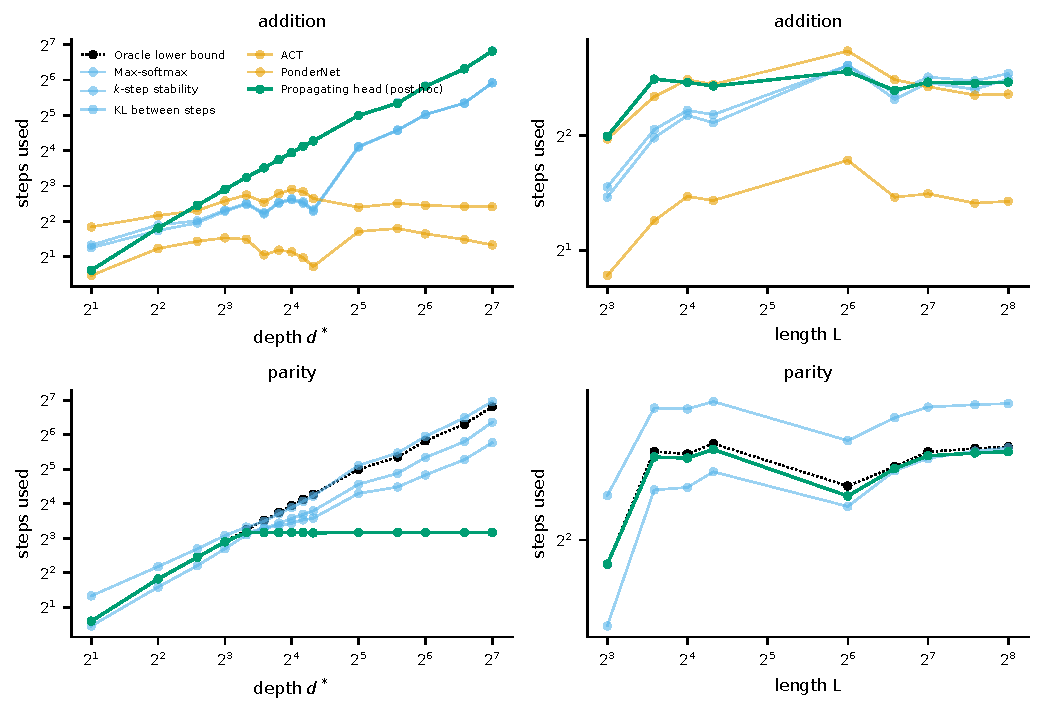
\includegraphics[width=0.78\linewidth]{figures/fig4_steps_vs_depth_length.pdf}
  \caption{Steps used against depth (left) and length (right). The light-cone bound (dotted) grows
  with depth only. Per-position rules on addition track it; pooled gates stay flat.}
  \label{fig:steps}
\end{figure}

\paragraph{Premature stopping is not premature error (H2).} Global convergence rules ($k$-step
stability and the KL divergence between steps) halt before $\mathrm{LB}(x)$ on 75\% of OOD-depth and
50\% of OOD-both addition instances (\cref{tab:premature}), yet remain 99.8\% accurate; their
premature-\emph{error} rate, pooled over the deep splits, is 0.1\%, against 18--23\% for ACT, PonderNet
and the joint pooled head. This is exactly the gap \cref{thm:lb} leaves open: the answers are
uncertified, but the data do not contain the flip partner. The backbone's default guess for a pending
digit is usually right, and while a carry wave is still travelling the hidden state keeps changing, so
convergence is a good proxy for completion. Parity shows the same effect in its sharpest form: one step
before the bound, a position has seen every bit of its segment and only the closing delimiter is
outside its window, so the natural guess (``no further bits'') is right on the actual input. This is
why the stable oracle and ACT can be accurate on parity OOD-depth while halting before the bound. The hidden-state-change rule, whose threshold is set on
short inputs, halts after about four steps on OOD-both and is correct on 42.7\%. On parity, where outputs
keep flipping as information arrives, confidence is misleading: max-softmax halts before the bound on
91\% of OOD-depth instances and is correct on 51\%; on OOD-both it is correct on 0.8\%. Only the KL rule
partly survives (94\% on OOD-depth, 57\% on OOD-both). Both H1 and H2 hold, so Gate G2 passes.

\begin{table}[t]
  \centering
  \caption{Premature-stop rate (\%): fraction of instances halted before the light-cone bound
  $\mathrm{LB}(x)$. Such answers are uncertified (\cref{thm:lb}), though not necessarily wrong.}
  \label{tab:premature}
  \scriptsize
  \setlength{\tabcolsep}{3pt}
  \resizebox{\linewidth}{!}{\begin{tabular}{lrrrr}
\toprule
 & \multicolumn{2}{c}{addition} & \multicolumn{2}{c}{parity} \\
 & OOD-depth & OOD-both & OOD-depth & OOD-both \\
\midrule
Fixed $T$ & 100.0 \tiny{[100.0, 100.0]} & 100.0 \tiny{[100.0, 100.0]} & 100.0 \tiny{[100.0, 100.0]} & 100.0 \tiny{[100.0, 100.0]} \\
Max-softmax & 0.0 \tiny{[0.0, 0.0]} & 0.0 \tiny{[0.0, 0.0]} & 90.8 \tiny{[89.9, 91.7]} & 98.2 \tiny{[97.5, 98.8]} \\
Entropy & 0.0 \tiny{[0.0, 0.0]} & 0.0 \tiny{[0.0, 0.0]} & 99.2 \tiny{[98.9, 99.5]} & 100.0 \tiny{[100.0, 100.0]} \\
$k$-step stability & 74.7 \tiny{[73.3, 76.0]} & 49.7 \tiny{[47.4, 51.9]} & 86.2 \tiny{[85.2, 87.3]} & 85.5 \tiny{[84.0, 87.1]} \\
KL between steps & 74.7 \tiny{[73.3, 76.0]} & 49.7 \tiny{[47.4, 51.9]} & 49.2 \tiny{[47.7, 50.7]} & 28.5 \tiny{[26.5, 30.6]} \\
Hidden-state change & 0.0 \tiny{[0.0, 0.0]} & 100.0 \tiny{[100.0, 100.0]} & 81.1 \tiny{[79.9, 82.3]} & 100.0 \tiny{[100.0, 100.0]} \\
Max confidence (Fan et al.) & 0.0 \tiny{[0.0, 0.0]} & 0.0 \tiny{[0.0, 0.0]} & 0.0 \tiny{[0.0, 0.0]} & 0.0 \tiny{[0.0, 0.0]} \\
Correctness head (post hoc) & 75.3 \tiny{[73.9, 76.6]} & 99.6 \tiny{[99.3, 99.9]} & 100.0 \tiny{[100.0, 100.0]} & 100.0 \tiny{[100.0, 100.0]} \\
ACT & 100.0 \tiny{[100.0, 100.0]} & 100.0 \tiny{[100.0, 100.0]} & -- & -- \\
PonderNet & 75.5 \tiny{[73.5, 77.4]} & 100.0 \tiny{[100.0, 100.0]} & -- & -- \\
Correctness head (joint) & -- & -- & -- & -- \\
v1 GLWM gate & -- & -- & -- & -- \\
Completion head (post hoc) & 0.0 \tiny{[0.0, 0.0]} & 0.0 \tiny{[0.0, 0.0]} & 100.0 \tiny{[100.0, 100.0]} & 100.0 \tiny{[100.0, 100.0]} \\
Propagating head (post hoc) & 0.7 \tiny{[0.4, 0.9]} & 0.1 \tiny{[0.0, 0.1]} & 100.0 \tiny{[100.0, 100.0]} & 100.0 \tiny{[100.0, 100.0]} \\
Completion head (joint) & -- & -- & -- & -- \\
Propagating head (joint) & -- & -- & -- & -- \\
\bottomrule
\end{tabular}}
\end{table}

\paragraph{Per-position certificates on addition (H3).} On addition every per-position rule halts at
the light-cone bound on every split, with no premature stops and at least 99\% accuracy: max-softmax,
entropy, and all four completion-head variants use 13.5 steps on OOD-depth and 75.4--75.6 on OOD-both,
against 13.5 and 75.4 for the oracle $\mathrm{LB}(x)$. The reason is visible in the theory: a pending
addition digit has two equally plausible outputs (carry or no carry), so a calibrated decoder is
uncertain at exactly the positions that are not yet determined, and the minimum over positions is a
local certificate in the sense of \cref{cor:local}. A linear probe recovers the pending bit from the
hidden state with AUC above 0.999 on every split (\cref{tab:probes}). Per-position confidence on
addition therefore already implements the automaton of \cref{prop:automaton}, and a learned completion
head adds nothing: G3, which required a 10-point gain over the best baseline, fails on addition by
construction.

\paragraph{Completion heads on parity learn the clock.} On parity all completion heads halt after about
nine steps regardless of depth, close to the largest training depth, and are correct on 31--34\% of
OOD-depth and 0\% of OOD-both instances, well below ACT and PonderNet on OOD-depth. The joint and
propagating variants behave the same. In training
every position is done by step 10, so ``late'' and ``done'' are indistinguishable, and the parity
backbone's hidden state encodes elapsed time well enough for the head to use it. The propagating head
was designed to wait for its neighbours, but nothing in the training data forces it to: a neighbour is
also always done by step 10. This is the same failure as the pooled gates, moved from the input length
to the step count. G3 fails on parity as well. Following the pre-registered pivot, we read the results
as a map of when simple signals suffice rather than as a win for a new halting method.

\paragraph{Decoupling (H4) and compute.} Training a completion head jointly changes the backbone's
step-averaged ID-val accuracy by less than 0.02 points on both tasks, so the auxiliary target does not
distort the task solution. Gates that reweight the task loss do: relative to the base model, ACT lowers
it by 34 points and the v1 gate by 17 points on addition (86 points for the v1 gate on parity), because
steps after the learned halting point receive little task gradient. In
FLOPs, a completion head costs one pointwise MLP per position and step, and the cost of every rule is
dominated by the number of steps it takes (\cref{fig:compute}). Wall-clock savings are smaller at our scale:
with online early exit on 512 OOD-depth instances, max-softmax takes 19.8\,ms against 23.8\,ms for the
full budget, while the completion heads take 23.8 and 28.3\,ms, because checking a rule after every step
(a host synchronisation plus re-batching) costs about as much as the steps it saves
(\cref{tab:probes}). Turning certified halting into latency savings needs fused halting checks or
larger models whose step cost dominates.

\paragraph{Ablations.} Removing input re-injection (recall) leaves OOD-depth intact but destroys
OOD-both (stable oracle 0.6\%). Halving the width to 64 lowers the stable oracle to 95.2\% but
max-softmax to 48.0\%: with less capacity the decoder's confidence stops tracking the pending state.
Two convolutions per step ($r=2$) reach 100\% on both (\cref{tab:probes}). Single seed each.
The accuracy-versus-steps trade-off of every threshold is shown in \cref{fig:tradeoff}, and premature stopping as a function of depth in
\cref{fig:premature_depth} (\cref{app:results}).

\section{Related work}
\label{sec:related}

\paragraph{Adaptive computation.} ACT \citep{graves2016act} and PonderNet \citep{banino2021pondernet}
learn a halting distribution that weights the task loss; Universal Transformers apply ACT per token
\citep{dehghani2019universal}, and SACT halts per spatial location \citep{figurnov2017sact}. These gates
are trained on the depths that occur in training, and we test them beyond those depths while separating
their sensitivity to length from their sensitivity to depth.

\paragraph{Recurrent models that extrapolate.} Neural GPUs learn long addition
\citep{kaiser2016neuralgpu} but fail on long carry chains that random inputs rarely contain
\citep{price2016extensions}, an observation DepthShift turns into a controlled split. Recurrent networks
extrapolate to harder instances by running more iterations
\citep{schwarzschild2021thinking,schwarzschild2021datasets,bansal2022endtoend}, with the count chosen by
the experimenter. Path independence makes convergence a usable signal \citep{anil2022path}, and
test-time training can select compute per sample \citep{bao2025stop}. Looped Transformers
\citep{giannou2023looped,yang2024looped,saunshi2025latent}, including those of \citet{fan2025looped}, need
ground-truth step counts in training and stop by oracle or maximum confidence at test time. AdRNNs
\citep{veerabadran2023adaptive} and ANIRA \citep{moosa2026anira} halt later on harder inputs, but there
harder also means larger, so depth and length are confounded. Implicit models solve for a fixed point
instead \citep{bai2019deq}.

\paragraph{Latent reasoning and recursive models.} Recurrent-depth language models exit per token from
the KL between steps \citep{geiping2025scaling}, Ouro learns an exit gate \citep{zhu2025ouro}, and Coconut
reasons in continuous latents \citep{hao2024coconut}. HRM \citep{wang2025hrm} and TRM
\citep{jolicoeur2025trm} train a pooled halting or correctness head, and HRM has been analysed by
\citet{ge2025hrm}. Recent diagnoses of halting in such models examine stochastic stopping schedules and
the link between loop count and length \citep{kuo2026stochastic}, post-hoc confidence that matches learned
gates \citep{popescu2026halting}, latent motion that drops after the first exact solution
\citep{krishna2026finish}, and states that encode computational status but grow less reliable with depth
\citep{liang2026horizon}. We add a per-instance depth with a provable lower bound, splits that separate
depth from length, and a local completion target.

\paragraph{Early exit, length generalisation and termination detection.} Early-exit networks halt on
confidence or patience \citep{teerapittayanon2016branchynet,elbayad2020depth,xin2020deebert,zhou2020pabee},
CALM adds calibrated guarantees \citep{schuster2022calm}, and language models can predict their own
correctness \citep{kadavath2022know}. Early exit for reasoning models relies on answer convergence or
dedicated predictors \citep{yang2025dynamic,liu2025convergence,nagle2026terminator,brown2026settle}. All of
these signals are pooled over the whole answer, whereas ours is per position and tested beyond the
training depth. Arithmetic and algorithmic tasks are standard probes of length generalisation
\citep{nogueira2021arithmetic,anil2022length,deletang2023chomsky,zhou2024raspl,mcleish2024embeddings}, and
shortcut solutions tie the depth a model needs to its architecture \citep{liu2023shortcuts}. Finally,
deciding from local information that a distributed computation has finished is a classic problem
\citep{dijkstra1980termination}; our completion heads learn such a detector for a neural computation, and
\cref{prop:automaton} shows that a local, size-invariant one exists for our tasks. \Cref{tab:related} in
\cref{app:results} compares the closest works property by property.

\paragraph{Limitations.} All runs use one consumer GPU and a five-hour training budget, which allowed two
seeds per method, single-seed ablations and a reduced tuning budget for PonderNet and the v1 gate. The
exact theory covers one-dimensional tasks with closed-form depth, no maze backbone passed G1, and the
parity backbone fails G1 on OOD-both; \cref{sec:limitations} discusses these points further.


\begin{ack}
Compute: one NVIDIA RTX 5070. GPU-hours are reported in \cref{app:details}.
\end{ack}

\bibliographystyle{plainnat}
\bibliography{references}

\appendix
\section{Limitations}
\label{sec:limitations}

\paragraph{Scale.} Every experiment runs on one consumer GPU (RTX 5070, 12\,GB). To fit a five-hour
training budget we cut the pre-registered grid, which called for five seeds per cell and a full maze
grid, down to two seeds per method, three single-seed ablations, and a smaller gate-tuning budget for
PonderNet and the v1 gate than was pre-registered (\texttt{PREREGISTRATION.md}, deviations). With two
seeds the accuracy intervals are little more than the seed range, and the pre-registered Wilcoxon tests
cannot reach significance. Some comparisons that we report as ties may separate with more seeds, and
small differences should not be read as effects.

\paragraph{Mazes.} We could not train a maze backbone that passes Gate G1 within the budget; when
stopped, it reached 3\% exact match on training-size mazes. We therefore make no claims about stopping
rules on mazes, and whether local completion heads help when information travels along corridors
remains open.

\paragraph{Tasks.} The exact theory covers one-dimensional tasks whose determining radius has a closed
form. Addition and segmented parity are deliberately simple, so that $\LB(x)$ is known for every
instance, and they are not representative of natural-language reasoning. Our conclusions concern
recurrent models with a known, local growth rate. They do not transfer directly to models with global
attention, whose light cone covers the whole input after a single step.

\paragraph{Backbone dependence.} A stopping rule can only be as good as the trajectory it reads. On
segmented parity the backbone fails Gate G1, since its stable-oracle accuracy out of distribution is
below the pre-registered 95\%, so the parity results measure stopping on an imperfect backbone. The
progressive loss was also seed-dependent on addition. Termination detection and depth extrapolation
are entangled: a rule that looks premature may in fact be reacting to a backbone that never resolves.

\paragraph{What the theory does not say.} \Cref{thm:lb} rules out \emph{certified} early answers, not
correct ones. A rule that halts before $\LB(x)$ can be right on the data distribution, and on addition
the convergence detectors often are, because a carry wave keeps the hidden state moving until it lands.
This is why we report the premature-stop and premature-error rates of \cref{eq:premature} separately,
and we do not claim that premature halting is always harmful.

\paragraph{Selection and thresholds.} Thresholds are tuned on ID-val by taking the cheapest setting
within 0.5 points of the best. A different tolerance would trade accuracy against steps differently.
The gate hyperparameters (the ACT ponder weight $\tauact$, the PonderNet prior $\lambda_p$ and the v1 gate
weight $\lambda$) were tuned on a small grid with one seed, and stronger tuning of the jointly trained
gates could narrow some of the gaps we report.

\paragraph{Broader impact.} This is basic research on small synthetic tasks. Better termination
detection lowers inference compute, and we see no direct path to harm beyond that of adaptive-compute
models in general.

\section{Proofs}
\label{app:proofs}

\begin{proof}[Proof of \cref{lem:cone}]
By induction on $t$. For $t=0$, $h_i^{(0)} = H(E(x_i))$ depends on $W_i^0(x) = (x_i)$ through a
function that does not depend on $i$. Assume the claim for $t$. The update for $h_i^{(t+1)}$ reads
$h_j^{(t)}$ and $e_j$ for $|j-i|\le r$. Each $h_j^{(t)}$ is a fixed function of
$W_j^{rt}(x) \subseteq W_i^{r(t+1)}(x)$ (padding positions contribute fixed values, which are also
determined by the window because the window records $\bot$), and each $e_j$ is a function of
$\tilde x_j\in W_i^{r}(x)$. Since $U$ is shared, $h_i^{(t+1)}$ is a fixed function of
$W_i^{r(t+1)}(x)$. The decoder is pointwise, which gives the statement about $\hat y$.
\end{proof}

\begin{proof}[Proof of \cref{thm:lb}]
Let $\rho = rt < \rho_i(x)$ (because $t < \lceil\rho_i/r\rceil$ implies $rt < \rho_i$). By minimality
of $\rho_i(x)$, position $i$ is not $\rho$-determined, so there is $(x', i')$ with
$W_{i'}^{\rho}(x') = W_i^{\rho}(x)$ and $y_{i'}(x')\ne y_i(x)$. By \cref{lem:cone},
$\hat y_{i'}^{(t)}(x') = \hat y_i^{(t)}(x)$, so this common prediction differs from at least one of the
two targets. Taking $i$ with $\rho_i(x) = d^*(x)$ gives the statement about $\mathrm{LB}(x)$.
\end{proof}

\begin{proof}[Proof of \cref{cor:local}]
Suppose position $i$ of $x$ commits at $t < \lceil\rho_i(x)/r\rceil$. Take the pair $(x', i')$ from
\cref{thm:lb}. The histories $h_i^{(0..t)}(x)$ and $h_{i'}^{(0..t)}(x')$ coincide by
\cref{lem:cone}, so position $i'$ of $x'$ raises its flag at the same step $t$ (it cannot have
raised it earlier, since $x$ would then have raised it earlier too) and commits the same prediction,
which is wrong for one of them. The input halts when all positions have committed, so it halts no
earlier than $\max_i\lceil\rho_i(x)/r\rceil = \mathrm{LB}(x)$.
\end{proof}

\begin{proof}[Proof of \cref{cor:length}]
At length $L$ the input with $a_j+b_j = 9$ for all $j<L$ has no stops, so $d^* = L+1$ by
\cref{prop:oracles}, and \cref{thm:lb} applies to the final carry position. Any $\tau(L)$ below
$\lceil (L+1)/r\rceil$ is therefore wrong on one member of the corresponding pair, and the same
argument applies to every input with $d^*(x) > r\tau(L)$. For uniformly random digits each position
is a non-stop with probability $1/10$, independently, so $d^*-1$ is the longest run of successes in
$L$ Bernoulli$(1/10)$ trials, which is $\log_{10} L + O_p(1)$ (the Erd\H{o}s--R\'enyi longest-run law).
\end{proof}

\begin{proof}[Proof of \cref{prop:oracles}]
\emph{Addition.} Output $i$ is $(a_i + b_i + c_i)\bmod 10$ for $i<L$ and $c_L$ for $i=L$, where $c_i$ is
the carry into $i$. If $s_i\ge 0$ is the nearest stop before $i$, then positions $s_i+1,\dots,i-1$
all have $a_j+b_j = 9$, so $c_i = c_{s_i+1} = \mathbb 1[a_{s_i}+b_{s_i}\ge 10]$. If there is no stop,
all positions $0,\dots,i-1$ sum to 9 and $c_i = c_0 = 0$.
\emph{Upper bound} ($\rho_i \le i - s_i$): the window of radius $i - s_i$ contains position $s_i$ (or the
boundary symbol $\bot$ at $-1$) and every position between, so it fixes $c_i$ and $(a_i,b_i)$, hence
$y_i$, for every $(x',i')$ sharing the window. A boundary symbol at relative offset $-(i-s_i)$ in
$x'$ forces $i' = i$, so the carry is 0 there too.
\emph{Lower bound} ($\rho_i \ge i - s_i$): take $\rho = i - s_i - 1$. The window contains positions
$i-\rho,\dots,i-1$, all summing to 9, and no boundary symbol on the left. Build $x'$ by
taking the window content, placing it at $i' = \rho+1$, and putting one digit pair at
position $0$ of $x'$ whose sum is $\ge 10$ if $c_i(x) = 0$ and $<9$ if $c_i(x)=1$ (the right-hand
part of the window is copied unchanged). Then $c_{i'}(x') = 1 - c_i(x)$, so $y_{i'}(x')\ne y_i(x)$.
\emph{Parity} is identical with ``delimiter'' for ``stop'' and the segment prefix parity for the carry:
flipping the bit just outside the window changes the parity.
\end{proof}

\begin{proof}[Proof of \cref{prop:automaton}]
\emph{Addition.} Each position stores its pair sum class and a carry-in $c_i\in\{0,1,?\}$, initially
$?$. Per step, position $i$ reads its left neighbour's carry-out, which is
$\mathbb 1[a_{i-1}+b_{i-1}\ge 10]$ if $i-1$ is a stop, $c_{i-1}$ if $a_{i-1}+b_{i-1}=9$, and $0$ if
the neighbour is the boundary $\bot$; it sets $c_i$ to that value if $c_i = ?$ and the value is
known. This update reads only radius-1 neighbours and is the same at every position and length.
By induction, $c_i$ becomes known exactly at step $i - s_i = \rho_i$ (step 1 at a stop's right
neighbour or at position 0, one more step for each 9 in between), and once known it equals the true
carry. The done flag is $\mathbb 1[c_i\ne ?]$ and the committed output is
$(a_i+b_i+c_i)\bmod 10$, which is correct. The input halts at $\max_i\rho_i = d^*(x) = \mathrm{LB}(x)$
for $r=1$. \emph{Parity}: the same construction with the segment prefix parity in place of the carry,
initialised to $0$ at delimiters.
\end{proof}

\section{Implementation details}
\label{app:details}

\paragraph{Training.} We use AdamW with learning rate $10^{-3}$ and weight decay $10^{-4}$, 300 warm-up
steps followed by cosine decay, and gradient clipping at 1.0. Training runs in fp32 with TF32 matrix
multiplies, which was faster than bf16 autocast for this launch-bound model on our GPU. For T1 and T2 the
backbone has width 128 and $r=1$ and is trained for 8000 iterations at batch size 512 with
$\Ttrain=20$. For T3 it has width 64 and $r=4$ and is trained for 5000 iterations at batch size 32, with
random dihedral augmentation and $\Ttrain=32$. Training batches are sampled on the GPU and filtered
against the ID-val and ID-test hashes. Base models use seeds 0--4 and jointly trained methods seeds 0--2
(T1/T2); mazes use seeds 0--1.

\paragraph{Gate hyperparameters.} Every jointly trained gate receives the same budget of three settings
on addition (seed 0). Among the settings within 0.5 points of the best ID-val accuracy, the one with the
fewest mean ID-val steps is used everywhere (\texttt{configs/tune\_gates.yaml}). The grids are
$\tauact\in\{10^{-3},10^{-2},10^{-1}\}$ for the ACT ponder weight,
$(\beta,\lambda_p)\in\{(0.01,0.1),(0.01,0.2),(0.1,0.05)\}$ for PonderNet, and
$\lambda\in\{10^{-3},10^{-2},10^{-1}\}$ for the compute weight of the v1 gate.

\paragraph{Post-hoc heads.} The post-hoc heads are fitted on the frozen backbone for 1500 iterations
(batch 256; batch 32 for mazes) on fresh training-distribution batches rolled out to $2\Ttrain$ steps,
with the backbone in bf16 autocast and the heads in fp32. We use Adam with learning rate
$2\cdot 10^{-3}$ and cosine decay. The pooled correctness head (TRM-style) predicts exact match from the
masked mean of the latent state, and the completion heads predict the target of \cref{eq:done} per
position.

\paragraph{Halting loop.} \Cref{alg:halt} spells out the halting rule of \cref{eq:halt} as it runs at
test time. Instances are processed in batches, and an instance leaves the batch as soon as it halts.

\begin{algorithm}[h]
  \caption{Halting with local completion heads (batched; halted instances leave the batch).}
  \label{alg:halt}
  \begin{algorithmic}[1]
    \Require input $x$, backbone $(E,H,U,D)$, completion head $c$, threshold $\theta$, budget $\Tmax$
    \State $e \gets E(x)$;\quad $h \gets H(e)$;\quad $p \gets \mathbf 0$
    \For{$t = 1,\dots,\Tmax$}
      \State $h \gets U(h, e)$;\quad $\yhat \gets \arg\max D(h)$
      \State $p \gets \sigma\bigl(c(h, p)\bigr)$ \Comment{per position; the pointwise head ignores $p$}
      \If{$\min_{i\ \text{valid}} p_i > \theta$ \textbf{or} $t = \Tmax$}
        \State \Return $(\yhat, t)$
      \EndIf
    \EndFor
  \end{algorithmic}
\end{algorithm}

\paragraph{Threshold grids.} Probability rules use the thresholds
\begin{equation*}
  \theta\in\{0.5,\,0.6,\,0.7,\,0.8,\,0.9,\,0.95,\,0.98,\,0.99,\,0.995,\,0.999,\,0.9999\}.
\end{equation*}
Entropy, KL and hidden-state change
use 19 log-spaced values in $[10^{-6},1]$, stability uses $k\in\{2,3,5\}$, ACT thresholds its cumulative
halting probability at $\{0.5,0.7,0.9,0.95,0.99\}$, PonderNet at $\{0.3,0.5,0.7,0.9,0.95,0.99\}$, and the
fixed-step rule uses $T\in\{1,\dots,\Tmax\}$. The test-time budget of each split is
\begin{equation*}
  \Tmax = \ceil*{\frac{\max_x \dstar(x)}{r}} + 16.
\end{equation*}

\paragraph{Metrics.} Besides accuracy, mean steps and the premature rates of \cref{eq:premature}, we
record several diagnostics. Let $t^{\mathrm{stab}}(x)$ be the first step from which the answer stays
correct, the step chosen by the stable oracle. \emph{Overthinking} is
$\tau(x)-t^{\mathrm{stab}}(x)$, averaged over correctly answered instances. \emph{Regret} is the accuracy
lost and the extra steps spent relative to the stable oracle, the latter measured on instances that the
oracle gets right. \emph{Depth tracking} is the Spearman correlation $\rho_S(\tau,\dstar)$, and
\emph{length leakage} the partial Spearman correlation $\rho_S(\tau, L\mid\dstar)$; a rule that halts at
$\LB(x)$ depends on depth alone and therefore leaks no length. Calibration is the 15-bin expected
calibration error of the per-position done probabilities.

\paragraph{Compute.} \Cref{tab:compute} lists the measured GPU time of each sweep.

\IfFileExists{tables/compute.tex}{\begin{table}[h]
\centering
\caption{Measured GPU time per sweep (RTX 5070; several runs shared the GPU, so wall-clock per run is higher than in isolation). Runs listed in more than one sweep are counted once per sweep.}
\label{tab:compute}
\small
\begin{tabular}{lrrr}
\toprule
Sweep & Runs & Train (h) & Eval (h) \\
\midrule
\texttt{ablations} & 3 & 0.6 & 0.2 \\
\texttt{main\_addition} & 8 & 2.6 & 0.6 \\
\texttt{main\_gates} & 12 & 5.2 & 1.3 \\
\texttt{main\_parity} & 8 & 2.4 & 1.3 \\
\texttt{pilot\_addition} & 8 & 2.4 & 1.1 \\
\texttt{tune\_gates} & 2 & 1.1 & 0.2 \\
\midrule
Total & 41 & 14.3 & 4.8 \\
\bottomrule
\end{tabular}
\end{table}}{}

\section{Additional results}
\label{app:results}

\paragraph{The v1 model, re-evaluated.} The original GLWM paper reported a mean of 1.05 steps with a gate
initialised to halt early. Re-running it with the evaluation of this paper (deduplicated test set,
exact match over all positions, \cref{tab:v1}) shows that both initialisations reach full accuracy,
the v1 initialisation uses 2.6 steps on average, and only 84\% of instances are already correct after
one step (\cref{fig:v1}). The earlier step count came from a halting criterion that stopped before the
answer had settled.

\begin{table}[h]
  \centering
  \caption{The v1 GLWM model with a fixed gate initialisation versus the original (v1) initialisation,
  evaluated on the deduplicated 4--8 digit test set.}
  \label{tab:v1}
  \small
  \begin{tabular}{lrrrrr}
\toprule
Gate init & Accuracy & Mean steps & Steps (4-digit) & Acc.\ at step 1 & MFLOPs/sample \\
\midrule
fixed & 1.0000 $\pm$ 0.0000 & 3.41 & 3.87 & 0.5888 & 7.50 \\
v1 & 1.0000 $\pm$ 0.0000 & 2.60 & 3.05 & 0.8405 & 7.02 \\
\bottomrule
\end{tabular}
\end{table}

\begin{figure}[h]
  \centering
  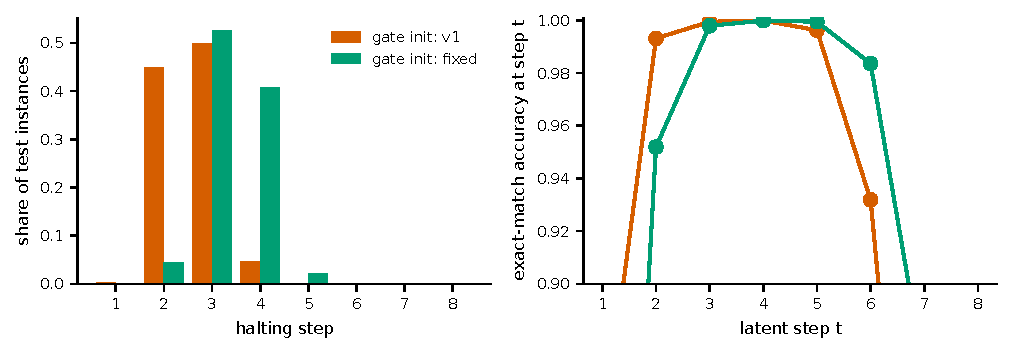
\includegraphics[width=\linewidth]{figures/figA_v1_corrected.pdf}
  \caption{v1 GLWM re-evaluated: halting steps (left) and exact-match accuracy at each latent step
  (right) for the two gate initialisations.}
  \label{fig:v1}
\end{figure}

\paragraph{Per-step accuracy of the backbones.} \Cref{fig:stepacc} shows exact-match accuracy at every
step for both objectives. On addition, accuracy on every split rises to its plateau and stays there:
once an answer is right it stays right. On parity, OOD-both accuracy peaks and then decays for both
objectives, so the stable oracle sits below 100\% and the backbone fails Gate G1.

\begin{figure}[h]
  \centering
  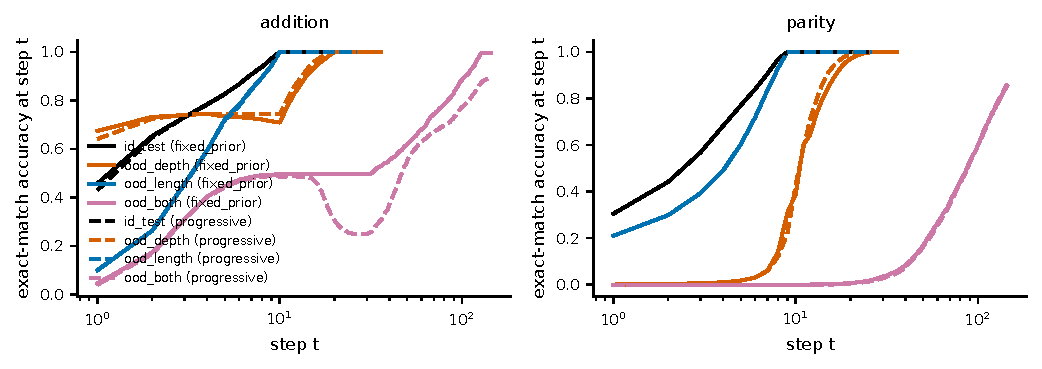
\includegraphics[width=\linewidth]{figures/figA_step_accuracy.pdf}
  \caption{Exact-match accuracy at step $t$ (mean over pilot seeds), fixed-prior (solid) and
  progressive (dashed) objectives.}
  \label{fig:stepacc}
\end{figure}

\begin{figure}[h]
  \centering
  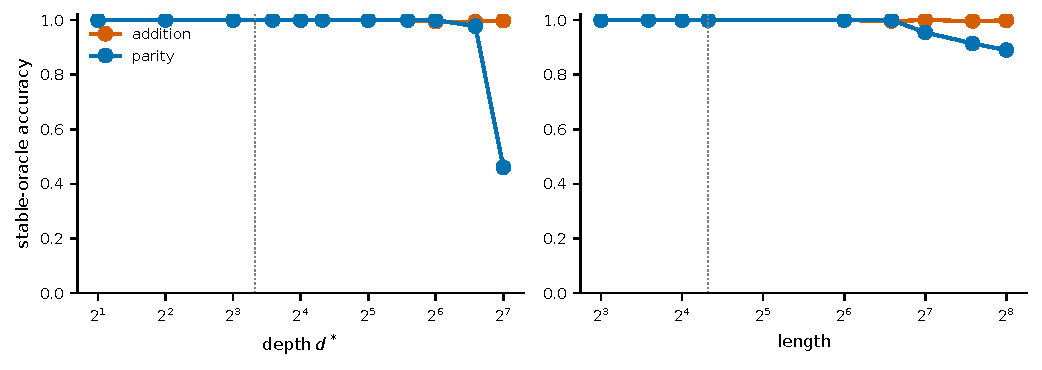
\includegraphics[width=\linewidth]{figures/fig3_oracle_vs_depth_length.pdf}
  \caption{Stable-oracle accuracy against depth (left) and length (right), pooled over splits; dotted
  lines mark the training maxima. Length alone costs nothing; accuracy on parity drops with depth.}
  \label{fig:oracle}
\end{figure}

\paragraph{Information travels at the light-cone speed.} \Cref{fig:posstep} shows, for one OOD-both
addition instance, which output positions are correct at which step, together with the per-position
lower bound $\rho_i$ from \cref{prop:oracles}. No position can be certified before its bound, and the
backbone's positions settle along a wave that follows it, travelling one position per step from each
stop. \Cref{fig:donespread} shows the done
probabilities of the two post-hoc completion heads on a deep instance: they switch on along the same
wave, after the bound.

\begin{figure}[h]
  \centering
  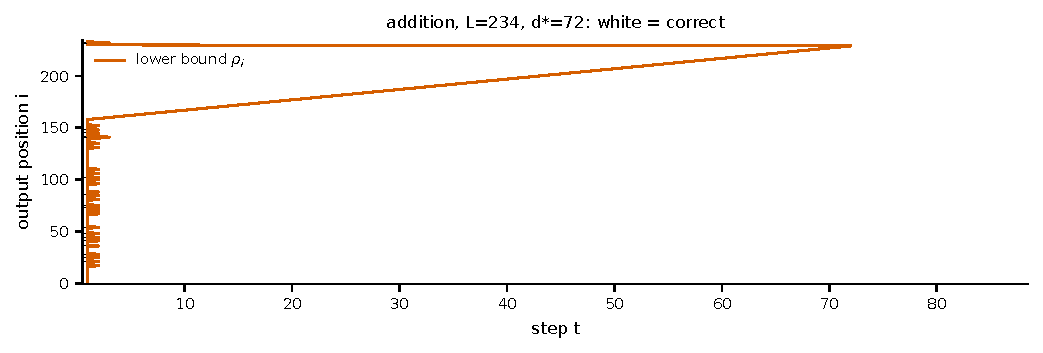
\includegraphics[width=\linewidth]{figures/figA_position_by_step.pdf}
  \caption{Correctness of every output position (rows) at every step (columns) for one OOD-both
  addition instance; white is correct. The orange line is the per-position lower bound $\rho_i$.}
  \label{fig:posstep}
\end{figure}

\begin{figure}[h]
  \centering
  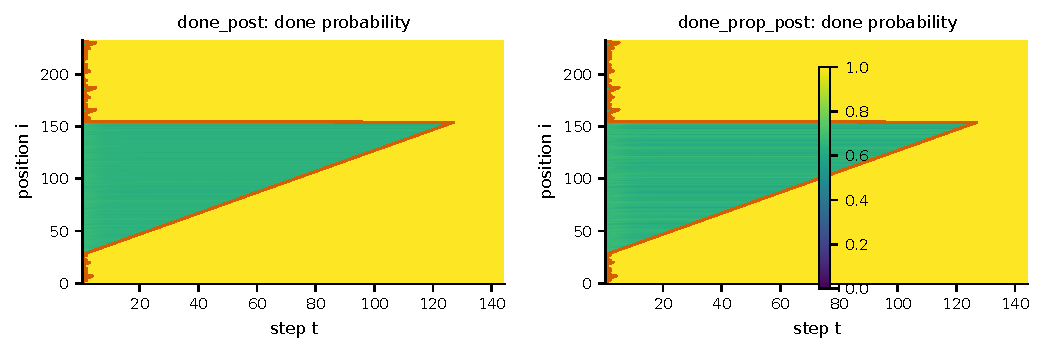
\includegraphics[width=\linewidth]{figures/figA_done_spread.pdf}
  \caption{Done probabilities of the post-hoc completion heads (pointwise, left; propagating, right) on a
  deep OOD-both addition instance, with the per-position lower bound in orange.}
  \label{fig:donespread}
\end{figure}

\paragraph{Linear probes.} A linear probe fitted on ID-val hidden states decodes whether a position is
still pending ($t < \rho_i$) from $h_i^{(t)}$, and transfers to OOD-depth and OOD-both without refitting
(\cref{tab:probes}). The backbone therefore represents the pending bit of the automaton in
\cref{prop:automaton}; whether a stopping rule uses it is a separate question.

\IfFileExists{tables/probes_ablations.tex}{\begin{table}[h]
\centering
\caption{Left: linear probe for the pending state (fitted on ID-val, seed-0 base model on addition). Middle: ablations on addition (seed 0; accuracy in \%). Right: CUDA-event latency for 512 OOD-depth instances with online early exit (median ms).}
\label{tab:probes}
\small
\begin{tabular}{lrr}
\toprule
Split & Acc. & AUC \\
\midrule
id-test & 100.0 & 1.000 \\
ood-depth & 100.0 & 1.000 \\
ood-both & 100.0 & 1.000 \\
\bottomrule
\end{tabular}\quad
\begin{tabular}{llrr}
\toprule
Ablation & Rule & OOD-depth & OOD-both \\
\midrule
main & max softmax & 100.0 & 99.8 \\
main & oracle stable & 100.0 & 99.6 \\
no recall & max softmax & 100.0 & 7.5 \\
no recall & oracle stable & 100.0 & 0.6 \\
r 2 & max softmax & 100.0 & 100.0 \\
r 2 & oracle stable & 100.0 & 100.0 \\
width 64 & max softmax & 100.0 & 48.0 \\
width 64 & oracle stable & 100.0 & 95.2 \\
\bottomrule
\end{tabular}\quad
\begin{tabular}{lr}
\toprule
Rule & ms \\
\midrule
fixed T (val-selected) & 7.4 \\
fixed T = T max & 23.8 \\
max softmax & 19.8 \\
done post & 23.8 \\
done prop post & 28.3 \\
\bottomrule
\end{tabular}
\end{table}
}{}

\paragraph{Measured compute.} \Cref{fig:compute} plots measured FLOPs per instance (from
\texttt{FlopCounterMode}, at the mean length of each split) against accuracy. The completion heads add
one small MLP per position and step; their cost is dominated by the number of steps they choose.

\begin{figure}[h]
  \centering
  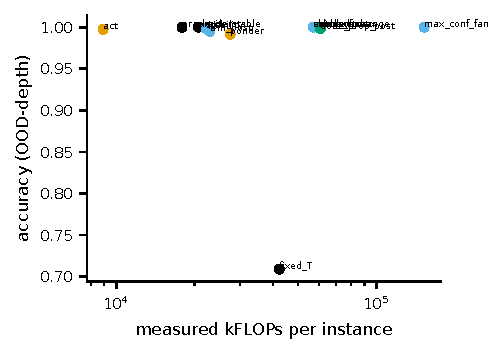
\includegraphics[width=0.6\linewidth]{figures/fig8_compute.pdf}
  \caption{Accuracy on addition OOD-depth against measured kFLOPs per instance for every stopping rule.}
  \label{fig:compute}
\end{figure}


\newpage
\section*{NeurIPS Paper Checklist}
\begin{enumerate}

\item {\bf Claims}
    \item[] Question: Do the main claims made in the abstract and introduction accurately reflect the paper's contributions and scope?
    \item[] Answer: \answerYes{} % Replace by \answerYes{}, \answerNo{}, or \answerNA{}.
    \item[] Justification: The abstract and \cref{sec:intro} state each claim with the experiment that tests it; \texttt{paper/claims\_map.md} maps every number to its source file.
    \item[] Guidelines:
    \begin{itemize}
        \item The answer NA means that the abstract and introduction do not include the claims made in the paper.
        \item The abstract and/or introduction should clearly state the claims made, including the contributions made in the paper and important assumptions and limitations. A No or NA answer to this question will not be perceived well by the reviewers. 
        \item The claims made should match theoretical and experimental results, and reflect how much the results can be expected to generalize to other settings. 
        \item It is fine to include aspirational goals as motivation as long as it is clear that these goals are not attained by the paper. 
    \end{itemize}

\item {\bf Limitations}
    \item[] Question: Does the paper discuss the limitations of the work performed by the authors?
    \item[] Answer: \answerYes{} % Replace by \answerYes{}, \answerNo{}, or \answerNA{}.
    \item[] Justification: \Cref{sec:limitations} discusses the tasks, the architecture class, the loose maze bound, and the cases where simple confidence rules suffice.
    \item[] Guidelines:
    \begin{itemize}
        \item The answer NA means that the paper has no limitation while the answer No means that the paper has limitations, but those are not discussed in the paper. 
        \item The authors are encouraged to create a separate "Limitations" section in their paper.
        \item The paper should point out any strong assumptions and how robust the results are to violations of these assumptions (e.g., independence assumptions, noiseless settings, model well-specification, asymptotic approximations only holding locally). The authors should reflect on how these assumptions might be violated in practice and what the implications would be.
        \item The authors should reflect on the scope of the claims made, e.g., if the approach was only tested on a few datasets or with a few runs. In general, empirical results often depend on implicit assumptions, which should be articulated.
        \item The authors should reflect on the factors that influence the performance of the approach. For example, a facial recognition algorithm may perform poorly when image resolution is low or images are taken in low lighting. Or a speech-to-text system might not be used reliably to provide closed captions for online lectures because it fails to handle technical jargon.
        \item The authors should discuss the computational efficiency of the proposed algorithms and how they scale with dataset size.
        \item If applicable, the authors should discuss possible limitations of their approach to address problems of privacy and fairness.
        \item While the authors might fear that complete honesty about limitations might be used by reviewers as grounds for rejection, a worse outcome might be that reviewers discover limitations that aren't acknowledged in the paper. The authors should use their best judgment and recognize that individual actions in favor of transparency play an important role in developing norms that preserve the integrity of the community. Reviewers will be specifically instructed to not penalize honesty concerning limitations.
    \end{itemize}

\item {\bf Theory assumptions and proofs}
    \item[] Question: For each theoretical result, does the paper provide the full set of assumptions and a complete (and correct) proof?
    \item[] Answer: \answerYes{} % Replace by \answerYes{}, \answerNo{}, or \answerNA{}.
    \item[] Justification: Assumptions are stated in \cref{sec:theory}; full proofs are in \cref{app:proofs}, and each result has an executable check in \texttt{tests/test\_theory.py}.
    \item[] Guidelines:
    \begin{itemize}
        \item The answer NA means that the paper does not include theoretical results. 
        \item All the theorems, formulas, and proofs in the paper should be numbered and cross-referenced.
        \item All assumptions should be clearly stated or referenced in the statement of any theorems.
        \item The proofs can either appear in the main paper or the supplemental material, but if they appear in the supplemental material, the authors are encouraged to provide a short proof sketch to provide intuition. 
        \item Inversely, any informal proof provided in the core of the paper should be complemented by formal proofs provided in appendix or supplemental material.
        \item Theorems and Lemmas that the proof relies upon should be properly referenced. 
    \end{itemize}

    \item {\bf Experimental result reproducibility}
    \item[] Question: Does the paper fully disclose all the information needed to reproduce the main experimental results of the paper to the extent that it affects the main claims and/or conclusions of the paper (regardless of whether the code and data are provided or not)?
    \item[] Answer: \answerYes{} % Replace by \answerYes{}, \answerNo{}, or \answerNA{}.
    \item[] Justification: \Cref{app:details} lists every hyperparameter, split and selection rule; one YAML config per run and \texttt{REPRODUCE.md} give the exact commands.
    \item[] Guidelines:
    \begin{itemize}
        \item The answer NA means that the paper does not include experiments.
        \item If the paper includes experiments, a No answer to this question will not be perceived well by the reviewers: Making the paper reproducible is important, regardless of whether the code and data are provided or not.
        \item If the contribution is a dataset and/or model, the authors should describe the steps taken to make their results reproducible or verifiable. 
        \item Depending on the contribution, reproducibility can be accomplished in various ways. For example, if the contribution is a novel architecture, describing the architecture fully might suffice, or if the contribution is a specific model and empirical evaluation, it may be necessary to either make it possible for others to replicate the model with the same dataset, or provide access to the model. In general. releasing code and data is often one good way to accomplish this, but reproducibility can also be provided via detailed instructions for how to replicate the results, access to a hosted model (e.g., in the case of a large language model), releasing of a model checkpoint, or other means that are appropriate to the research performed.
        \item While NeurIPS does not require releasing code, the conference does require all submissions to provide some reasonable avenue for reproducibility, which may depend on the nature of the contribution. For example
        \begin{enumerate}
            \item If the contribution is primarily a new algorithm, the paper should make it clear how to reproduce that algorithm.
            \item If the contribution is primarily a new model architecture, the paper should describe the architecture clearly and fully.
            \item If the contribution is a new model (e.g., a large language model), then there should either be a way to access this model for reproducing the results or a way to reproduce the model (e.g., with an open-source dataset or instructions for how to construct the dataset).
            \item We recognize that reproducibility may be tricky in some cases, in which case authors are welcome to describe the particular way they provide for reproducibility. In the case of closed-source models, it may be that access to the model is limited in some way (e.g., to registered users), but it should be possible for other researchers to have some path to reproducing or verifying the results.
        \end{enumerate}
    \end{itemize}


\item {\bf Open access to data and code}
    \item[] Question: Does the paper provide open access to the data and code, with sufficient instructions to faithfully reproduce the main experimental results, as described in supplemental material?
    \item[] Answer: \answerYes{} % Replace by \answerYes{}, \answerNo{}, or \answerNA{}.
    \item[] Justification: All code, configs, frozen-split hashes and the analysis notebooks are released; the data are generated from fixed seeds.
    \item[] Guidelines:
    \begin{itemize}
        \item The answer NA means that paper does not include experiments requiring code.
        \item Please see the NeurIPS code and data submission guidelines (\url{https://nips.cc/public/guides/CodeSubmissionPolicy}) for more details.
        \item While we encourage the release of code and data, we understand that this might not be possible, so “No” is an acceptable answer. Papers cannot be rejected simply for not including code, unless this is central to the contribution (e.g., for a new open-source benchmark).
        \item The instructions should contain the exact command and environment needed to run to reproduce the results. See the NeurIPS code and data submission guidelines (\url{https://nips.cc/public/guides/CodeSubmissionPolicy}) for more details.
        \item The authors should provide instructions on data access and preparation, including how to access the raw data, preprocessed data, intermediate data, and generated data, etc.
        \item The authors should provide scripts to reproduce all experimental results for the new proposed method and baselines. If only a subset of experiments are reproducible, they should state which ones are omitted from the script and why.
        \item At submission time, to preserve anonymity, the authors should release anonymized versions (if applicable).
        \item Providing as much information as possible in supplemental material (appended to the paper) is recommended, but including URLs to data and code is permitted.
    \end{itemize}


\item {\bf Experimental setting/details}
    \item[] Question: Does the paper specify all the training and test details (e.g., data splits, hyperparameters, how they were chosen, type of optimizer, etc.) necessary to understand the results?
    \item[] Answer: \answerYes{} % Replace by \answerYes{}, \answerNo{}, or \answerNA{}.
    \item[] Justification: \Cref{sec:benchmark,sec:method} and \cref{app:details} give splits, objectives, optimiser, schedules, threshold grids and the ID-val selection rule.
    \item[] Guidelines:
    \begin{itemize}
        \item The answer NA means that the paper does not include experiments.
        \item The experimental setting should be presented in the core of the paper to a level of detail that is necessary to appreciate the results and make sense of them.
        \item The full details can be provided either with the code, in appendix, or as supplemental material.
    \end{itemize}

\item {\bf Experiment statistical significance}
    \item[] Question: Does the paper report error bars suitably and correctly defined or other appropriate information about the statistical significance of the experiments?
    \item[] Answer: \answerYes{} % Replace by \answerYes{}, \answerNo{}, or \answerNA{}.
    \item[] Justification: 95\% bootstrap confidence intervals over instances (clustered by seed), Wilcoxon tests across seeds and Holm correction; \cref{sec:experiments}.
    \item[] Guidelines:
    \begin{itemize}
        \item The answer NA means that the paper does not include experiments.
        \item The authors should answer "Yes" if the results are accompanied by error bars, confidence intervals, or statistical significance tests, at least for the experiments that support the main claims of the paper.
        \item The factors of variability that the error bars are capturing should be clearly stated (for example, train/test split, initialization, random drawing of some parameter, or overall run with given experimental conditions).
        \item The method for calculating the error bars should be explained (closed form formula, call to a library function, bootstrap, etc.)
        \item The assumptions made should be given (e.g., Normally distributed errors).
        \item It should be clear whether the error bar is the standard deviation or the standard error of the mean.
        \item It is OK to report 1-sigma error bars, but one should state it. The authors should preferably report a 2-sigma error bar than state that they have a 96\% CI, if the hypothesis of Normality of errors is not verified.
        \item For asymmetric distributions, the authors should be careful not to show in tables or figures symmetric error bars that would yield results that are out of range (e.g. negative error rates).
        \item If error bars are reported in tables or plots, The authors should explain in the text how they were calculated and reference the corresponding figures or tables in the text.
    \end{itemize}

\item {\bf Experiments compute resources}
    \item[] Question: For each experiment, does the paper provide sufficient information on the computer resources (type of compute workers, memory, time of execution) needed to reproduce the experiments?
    \item[] Answer: \answerYes{} % Replace by \answerYes{}, \answerNo{}, or \answerNA{}.
    \item[] Justification: One RTX 5070; GPU-hours per sweep are reported in \cref{app:details}.
    \item[] Guidelines:
    \begin{itemize}
        \item The answer NA means that the paper does not include experiments.
        \item The paper should indicate the type of compute workers CPU or GPU, internal cluster, or cloud provider, including relevant memory and storage.
        \item The paper should provide the amount of compute required for each of the individual experimental runs as well as estimate the total compute. 
        \item The paper should disclose whether the full research project required more compute than the experiments reported in the paper (e.g., preliminary or failed experiments that didn't make it into the paper). 
    \end{itemize}
    
\item {\bf Code of ethics}
    \item[] Question: Does the research conducted in the paper conform, in every respect, with the NeurIPS Code of Ethics \url{https://neurips.cc/public/EthicsGuidelines}?
    \item[] Answer: \answerYes{} % Replace by \answerYes{}, \answerNo{}, or \answerNA{}.
    \item[] Justification: The work uses synthetic data only and follows the NeurIPS Code of Ethics.
    \item[] Guidelines:
    \begin{itemize}
        \item The answer NA means that the authors have not reviewed the NeurIPS Code of Ethics.
        \item If the authors answer No, they should explain the special circumstances that require a deviation from the Code of Ethics.
        \item The authors should make sure to preserve anonymity (e.g., if there is a special consideration due to laws or regulations in their jurisdiction).
    \end{itemize}


\item {\bf Broader impacts}
    \item[] Question: Does the paper discuss both potential positive societal impacts and negative societal impacts of the work performed?
    \item[] Answer: \answerNA{} % Replace by \answerYes{}, \answerNo{}, or \answerNA{}.
    \item[] Justification: Foundational research on halting in small synthetic-task models; we see no direct societal impact beyond general efficiency of iterative models.
    \item[] Guidelines:
    \begin{itemize}
        \item The answer NA means that there is no societal impact of the work performed.
        \item If the authors answer NA or No, they should explain why their work has no societal impact or why the paper does not address societal impact.
        \item Examples of negative societal impacts include potential malicious or unintended uses (e.g., disinformation, generating fake profiles, surveillance), fairness considerations (e.g., deployment of technologies that could make decisions that unfairly impact specific groups), privacy considerations, and security considerations.
        \item The conference expects that many papers will be foundational research and not tied to particular applications, let alone deployments. However, if there is a direct path to any negative applications, the authors should point it out. For example, it is legitimate to point out that an improvement in the quality of generative models could be used to generate deepfakes for disinformation. On the other hand, it is not needed to point out that a generic algorithm for optimizing neural networks could enable people to train models that generate Deepfakes faster.
        \item The authors should consider possible harms that could arise when the technology is being used as intended and functioning correctly, harms that could arise when the technology is being used as intended but gives incorrect results, and harms following from (intentional or unintentional) misuse of the technology.
        \item If there are negative societal impacts, the authors could also discuss possible mitigation strategies (e.g., gated release of models, providing defenses in addition to attacks, mechanisms for monitoring misuse, mechanisms to monitor how a system learns from feedback over time, improving the efficiency and accessibility of ML).
    \end{itemize}
    
\item {\bf Safeguards}
    \item[] Question: Does the paper describe safeguards that have been put in place for responsible release of data or models that have a high risk for misuse (e.g., pretrained language models, image generators, or scraped datasets)?
    \item[] Answer: \answerNA{} % Replace by \answerYes{}, \answerNo{}, or \answerNA{}.
    \item[] Justification: No pretrained language or image models or scraped data are released.
    \item[] Guidelines:
    \begin{itemize}
        \item The answer NA means that the paper poses no such risks.
        \item Released models that have a high risk for misuse or dual-use should be released with necessary safeguards to allow for controlled use of the model, for example by requiring that users adhere to usage guidelines or restrictions to access the model or implementing safety filters. 
        \item Datasets that have been scraped from the Internet could pose safety risks. The authors should describe how they avoided releasing unsafe images.
        \item We recognize that providing effective safeguards is challenging, and many papers do not require this, but we encourage authors to take this into account and make a best faith effort.
    \end{itemize}

\item {\bf Licenses for existing assets}
    \item[] Question: Are the creators or original owners of assets (e.g., code, data, models), used in the paper, properly credited and are the license and terms of use explicitly mentioned and properly respected?
    \item[] Answer: \answerYes{} % Replace by \answerYes{}, \answerNo{}, or \answerNA{}.
    \item[] Justification: PyTorch (BSD) and the arXiv metadata used for the bibliography are credited; maze data are generated by our own code.
    \item[] Guidelines:
    \begin{itemize}
        \item The answer NA means that the paper does not use existing assets.
        \item The authors should cite the original paper that produced the code package or dataset.
        \item The authors should state which version of the asset is used and, if possible, include a URL.
        \item The name of the license (e.g., CC-BY 4.0) should be included for each asset.
        \item For scraped data from a particular source (e.g., website), the copyright and terms of service of that source should be provided.
        \item If assets are released, the license, copyright information, and terms of use in the package should be provided. For popular datasets, \url{paperswithcode.com/datasets} has curated licenses for some datasets. Their licensing guide can help determine the license of a dataset.
        \item For existing datasets that are re-packaged, both the original license and the license of the derived asset (if it has changed) should be provided.
        \item If this information is not available online, the authors are encouraged to reach out to the asset's creators.
    \end{itemize}

\item {\bf New assets}
    \item[] Question: Are new assets introduced in the paper well documented and is the documentation provided alongside the assets?
    \item[] Answer: \answerYes{} % Replace by \answerYes{}, \answerNo{}, or \answerNA{}.
    \item[] Justification: The DepthShift generators and stopping-rule library are documented in the repository README and \texttt{REPRODUCE.md}.
    \item[] Guidelines:
    \begin{itemize}
        \item The answer NA means that the paper does not release new assets.
        \item Researchers should communicate the details of the dataset/code/model as part of their submissions via structured templates. This includes details about training, license, limitations, etc. 
        \item The paper should discuss whether and how consent was obtained from people whose asset is used.
        \item At submission time, remember to anonymize your assets (if applicable). You can either create an anonymized URL or include an anonymized zip file.
    \end{itemize}

\item {\bf Crowdsourcing and research with human subjects}
    \item[] Question: For crowdsourcing experiments and research with human subjects, does the paper include the full text of instructions given to participants and screenshots, if applicable, as well as details about compensation (if any)? 
    \item[] Answer: \answerNA{} % Replace by \answerYes{}, \answerNo{}, or \answerNA{}.
    \item[] Justification: No crowdsourcing or human subjects.
    \item[] Guidelines:
    \begin{itemize}
        \item The answer NA means that the paper does not involve crowdsourcing nor research with human subjects.
        \item Including this information in the supplemental material is fine, but if the main contribution of the paper involves human subjects, then as much detail as possible should be included in the main paper. 
        \item According to the NeurIPS Code of Ethics, workers involved in data collection, curation, or other labor should be paid at least the minimum wage in the country of the data collector. 
    \end{itemize}

\item {\bf Institutional review board (IRB) approvals or equivalent for research with human subjects}
    \item[] Question: Does the paper describe potential risks incurred by study participants, whether such risks were disclosed to the subjects, and whether Institutional Review Board (IRB) approvals (or an equivalent approval/review based on the requirements of your country or institution) were obtained?
    \item[] Answer: \answerNA{} % Replace by \answerYes{}, \answerNo{}, or \answerNA{}.
    \item[] Justification: No human subjects.
    \item[] Guidelines:
    \begin{itemize}
        \item The answer NA means that the paper does not involve crowdsourcing nor research with human subjects.
        \item Depending on the country in which research is conducted, IRB approval (or equivalent) may be required for any human subjects research. If you obtained IRB approval, you should clearly state this in the paper. 
        \item We recognize that the procedures for this may vary significantly between institutions and locations, and we expect authors to adhere to the NeurIPS Code of Ethics and the guidelines for their institution. 
        \item For initial submissions, do not include any information that would break anonymity (if applicable), such as the institution conducting the review.
    \end{itemize}

\item {\bf Declaration of LLM usage}
    \item[] Question: Does the paper describe the usage of LLMs if it is an important, original, or non-standard component of the core methods in this research? Note that if the LLM is used only for writing, editing, or formatting purposes and does not impact the core methodology, scientific rigorousness, or originality of the research, declaration is not required.
    %this research? 
    \item[] Answer: \answerYes{} % Replace by \answerYes{}, \answerNo{}, or \answerNA{}.
    \item[] Justification: An AI coding assistant was used to write code and draft text under the author's direction; all results come from the released code and were checked by the author. LLMs are not part of the method.
    \item[] Guidelines:
    \begin{itemize}
        \item The answer NA means that the core method development in this research does not involve LLMs as any important, original, or non-standard components.
        \item Please refer to our LLM policy (\url{https://neurips.cc/Conferences/2025/LLM}) for what should or should not be described.
    \end{itemize}

\end{enumerate}


\end{document}
